\subsection{Hierarchical model using cross-national, cross-sectoral data}

To measure corruption, presence of FDI, and treatment of firms across countries, I utilize the World Bank's Enterprise Survey (ES), which includes a wealth of firm-level data across 125 countries, spanning various topics from investment, labor, to business-government relation \citep{WorldBank2015}. The Enterprise Survey uses stratified random sampling (using three strata: firm size, business sector, and region) in order to ensure representativeness. The survey data comes from face-to-face interviews with upper management and is anonymized to ensure confidentiality at all times.\footnote{For more on the methodology of the Enterprise Survey, visit \url{http://www.enterprisesurveys.org/methodology}} This dataset has a wealth of firm-level data that helps us operationalize key concepts as detailed below.

Recall our hypothesis:

\begin{quote}
Hypothesis: The presence of large FDI firms in corrupt countries is associated with a large gap in the government's treatment of domestic firms and foreign firms in those countries.
\end{quote}

\begin{quote}
Hypothesis: The presence of large FDI firms in corrupt sectors is associated with a large gap in the government's treatment of domestic firms and foreign firms in those sectors.
\end{quote}

Operationalization of independent variables:
\begin{itemize}
\item FDI in countries: available via UNCTAD data on FDI flows and stocks to countries.

\item FDI in sectors: available via the Enterprises Survey dataset. The ``largeness'' of FDI firms can be measured by constructing a Herfindahl-Hirschman Index based on the size of sale, labor, or capital of firms. This allows us to calibrate the ``largeness'' of FDI firms according to the size of the host country's market.

\item Corruption: can be measured in two ways. 1) Firms' perception about corruption as an obstacle. This measure is frequently used but not accurate since firms' perception of corruption depends not only on the level of corruption but also the characteristics of firms. 2) Hard measure of prevalence and depth of bribes, e.g. ``Was an informal payment expected or request (when applying for a license)?'', ``How much do establishments like this one give in informal payments?'' 
\end{itemize}

Operationalization of dependent variable (i.e. the gap in the government's treatment of domestic firms and foreign firms):
\begin{itemize}
\item The gap can be measured by hard measures of business experience. It is important to choose aspects of the business experience that can be \textit{selectively} targeted by the government, e.g. tax rate, time spent dealing with inspectors, etc. In contrast, other aspects, such as quality of the labor force, days without electricity, etc. are harder to be targeted to a certain type of firms. These aspects can serve as the dependent variables in a placebo test.

It is important to note that this design does not suffer from selection bias. In the large literature using FDI survey data, it is impossible to control for the fact that the foreign firms that show up in the sample are the ones that self-select into investing. However, this is not an issue for our design. Because foreign firms that self-select into investing are more likely to be similar to domestic firms than foreign firms that do not, the \textit{observed} gap in the business experience of foreign and domestic firms in the sample is biased downwards and against our hypothesis.
\end{itemize}

\subsection{Cross-sectoral and sub-national variation in Vietnam}

As mentioned earlier, despite the wealth of firm-level, cross-national data in the ES dataset, its measure of corruption is still plagued by a host of measurement issues. Asking directly about firms' experience with corruption is unlikely to get an accurate answer due to sensitivity bias \citep{Coutts2011}. Researchers, including the ES team, often address this problem by framing the question about the experience with corruption of ``firms like yours.'' However, with this technique, firms may not read between the lines and actually answer about the experience of others \citep{Ahart2004}.

I remedy these problems with a research design focusing on the case of Vietnam, taking advantage by a survey list experiment by \citet{Malesky2015}, which uses unmatched count technique to accurately measure the experience of firms with corruption while avoiding sensitivity bias.

Recall the hypothesis:

\begin{quote}
Hypothesis: The presence of large FDI firms in provinces whose leaders are not interested in promotion is associated with a large gap in the government's treatment of domestic and foreign firms.
\end{quote}

Operationalization of independent variables:
\begin{itemize}
\item FDI in province: provincial statistics of FDI flow (government website)
\item FDI in sectors: government website
\item Corruption: list experiment \citep{Malesky2015}
\item Interest in promotion: 
\begin{itemize}
	\item base chance of promotion: years until retirement (retirement age is 60 for male, 55 for female)
	\item appearance in centrally controlled newspapers as a proxy for the decision to pursue promotion
\end{itemize}
\end{itemize}

Operationalization of the dependent variable, i.e. the gap in the government's treatment of the foreign and domestic firms
\begin{itemize}
	\item PCI survey question: ``Do you think that the provincial officials prefer FDI?'' (Question H3)
	\item The gap in the perception of domestic and foreign firms regarding the pro-activeness of the government in helping business (Form H for domestic firms and Form J for foreign firms)
	\item Hard measures of the business experience (similar to the Enterprises Survey)
\end{itemize}

\begin{figure}[!ht]
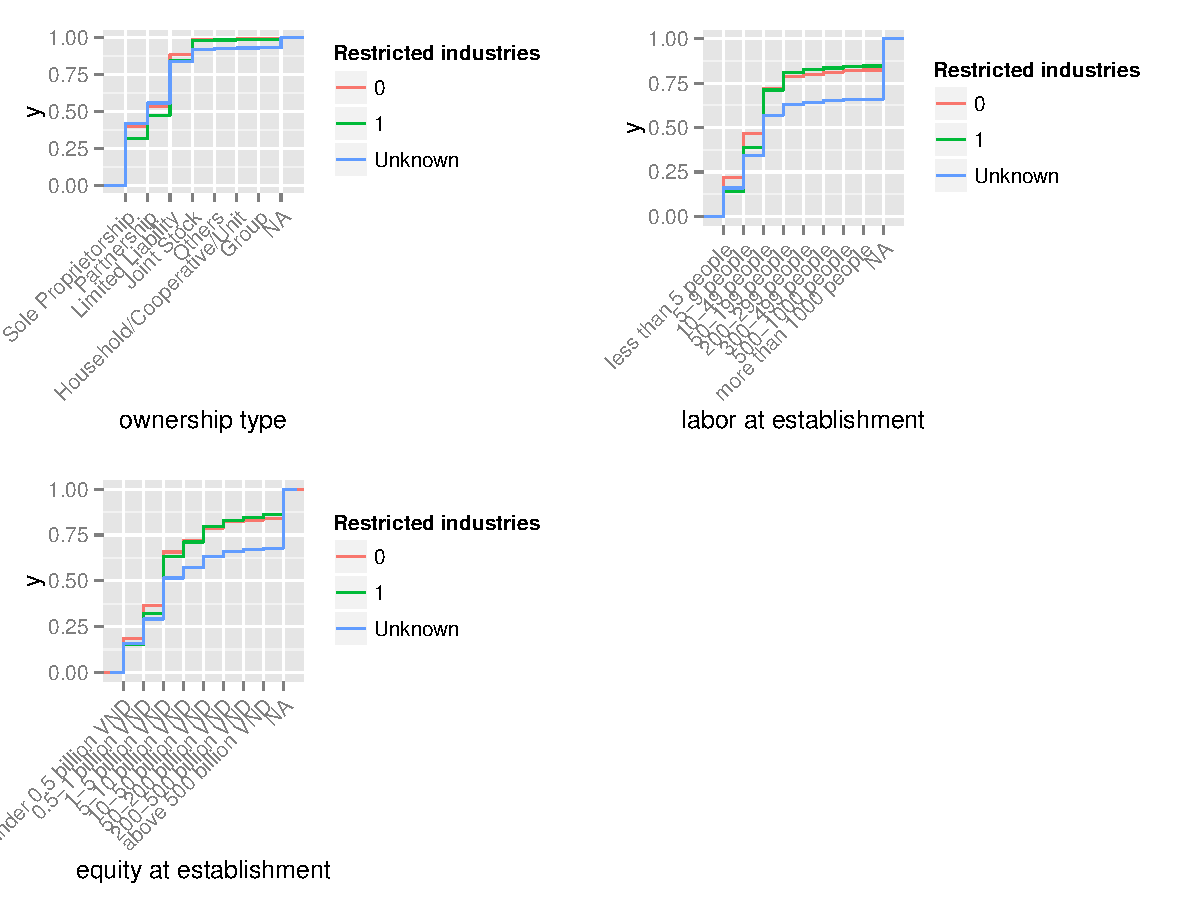
\includegraphics[width=\textwidth, height=\textheight,keepaspectratio]{../figure/by_restrict_owner-labor-equity}
\caption{The relationship between a province's FDI bias and attitude towards the private sector}
\label{fig:by_restrict_owner}
\end{figure}

\begin{figure}[!ht]
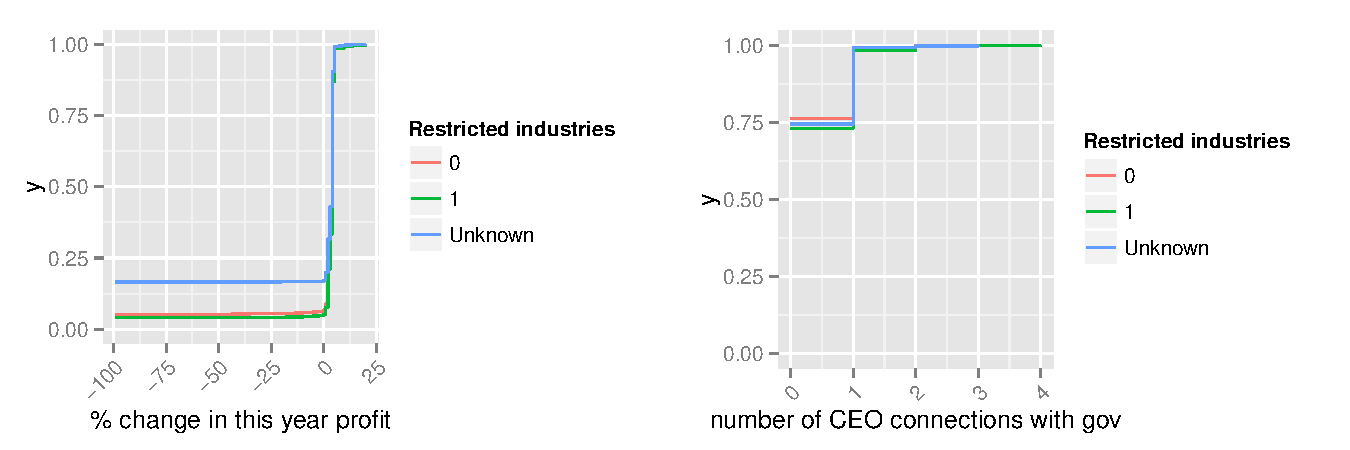
\includegraphics[width=\textwidth, height=\textheight,keepaspectratio]{../figure/by_restrict_performance-connection}
\caption{The relationship between a province's FDI bias and attitude towards the private sector}
\label{fig:by_restrict_performance}
\end{figure}

\subsection{Conjoint analysis}

The crucial causal mechanism in my theory is the utility calculation of provincial officials. However, observational data does not allow us to fully examine this key step because what the officials truly want may not be fulfilled due to external factors and thus cannot be observed. Furthermore, what an official wants from a FDI firm is often hard to tease out completely. A big FDI firm is an attractive source of rent, but it also brings job and technology. Indeed, perhaps this high correlation is precisely why it is so easy for officials to extract rent from FDI under the guise of promoting economic development.

To truly get at the utility calculation of provincial officials, I plan to conduct a survey experiment using conjoint analysis to ask provincial officials about their preference between two hypothetical FDI firms \citep{Hainmueller2014}. The characteristics of these firms will be randomly varied across five dimensions: 1) industry, 2) size of labor force, 3) capital, 4) technology age, and 5) land, which proxies for corruption opportunities, since this is a key resource to firm that is controlled by provincial officials. If desired, it is possible to:
\begin{itemize}
\item adjust the design so that implausible hypotheticals will not appear (i.e. there should not be a high-tech company with very small capital).
\item randomize the ordering of the characteristics between respondents to test for the ordering effect (i.e. knowing a firm's industry first changes how the respondent thinks about the other characteristics)
\end{itemize}

I am mainly interested in the ``average marginal component effect'' (AMCE) of \textit{land}, which is the marginal effect of \textit{land} on the likelihood of a project being preferred, averaged over the distribution of all the other components. This allows us to back-out what provincial officials truly want from a FDI project.

\subsubsection{Conjoint analysis design}
Please read the following description carefully. Then, please indicate which project you prefer to grant investment license (cap giay phep dau tu).

\begin{center}
  \begin{tabular}{ c | c | c }
    \hline
     & Project 1 (Du an 1) & Project 2 (Du an 1) \\ \hline
    Industry &  &  \\ \hline
    Labor force &  &  \\ \hline
    Capital &  &  \\ \hline
    Land &  &  \\ \hline
    Technology age &  &  \\ \hline
    \hline
  \end{tabular}
\end{center}

If you have to choose, which project do you prefer to grant investment license? Project 1 / Project 2

\begin{itemize}
\item Industry: textile, electronics, automobile, consumer product
\item Labor force: 5, 50, 100, 200, 500 employees
\item Capital:
\item Land:
\item Technology age: 
\end{itemize}
